\documentclass[12pt,a4paper]{article}
\usepackage[utf8]{inputenc}
\usepackage[T1]{fontenc}
\usepackage[english, ngerman]{babel}
\usepackage{graphicx}
\usepackage{fancyhdr}
\usepackage{geometry}
\usepackage{setspace}
\usepackage{titlesec}
\usepackage{enumitem}
\usepackage{lmodern}
\usepackage{hyperref}
\usepackage{bookmark}
\usepackage{multicol}
\usepackage{multicol}
\usepackage{titlesec}

\setlength{\headheight}{15pt}

% variables
\newcommand{\AuthorName}{Sebastian Simon (Hollow)}

\geometry{left=2.5cm, right=2.5cm, top=2.5cm, bottom=2.5cm}
\pagestyle{fancy}
\fancyhf{}
\rhead{Autor: \AuthorName}
\lhead{Charakterbook: Kagami Kagamiya}
\cfoot{\thepage}

\titleformat{\section}{\normalfont\Large\bfseries}{\thesection}{1em}{}
\titleformat{\subsection}{\normalfont\large\bfseries}{\thesubsection}{1em}{}

\hypersetup{
    colorlinks=true,
    linkcolor=black,
    urlcolor=blue
}

\begin{document}

% Deckblatt
\begin{titlepage}
    \centering
    \vspace*{2cm}
    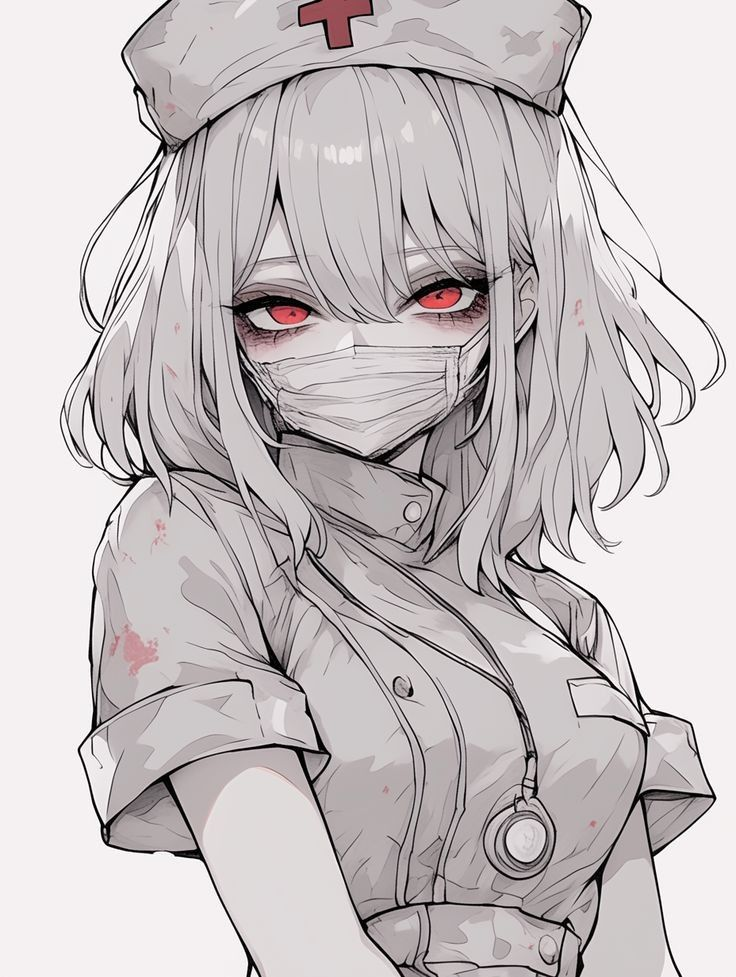
\includegraphics[width=0.7\textwidth]{kagami.jpg}\\[1.5cm]
    {\Huge\bfseries Kagami Kagamiya}\\[0.5cm]
    {\Large Für die Kampagne von Joshua}\\[2cm]
    \vfill
    \textsc{Autor:} \AuthorName \\
    \vfill
    \today
\end{titlepage}

\newpage
\tableofcontents
\newpage

% Steckbrief
\section{Steckbrief}
\begin{description}[style=nextline]
  \item[Name:] Kagami Kagamiya
  \item[Rasse:] Elfe (Albino)
  \item[Alter:] 25 Jahre
  \item[Größe:] 168 cm
  \item[Gewicht:] 59 kg   
  \item[Herkunft:] Dorf nahe [Stadt], im Land [Land] auf dem Kontinent [Kontinent]
  \item[Beruf:] Apothekerin und freiwillige Ärztin
  \item[Aussehen:] Blasses weißes Haar, rote Augen, meist mit Maske. Trägt schlichte, praktische Kleidung.
  \item[Charakter:] Ruhig, gelassen – aber leidenschaftlich und neugierig, wenn es um Medizin geht.
  \item[Glaube:] Atheistin
  \item[Ziele:] Wissen über Medizin erweitern, Krankheiten verstehen und heilen, mehr über die Welt lernen
\end{description}

\newpage

% TODO Geschwister ??

% Backgroundstory teil
\section{Backgroundstory}

Kagami Kagamiya wurde im kleinen, abgeschiedenen Dorf [Dorf] geboren, eingebettet zwischen alten Bäumen und Nebelschwaden eines uralten Waldes. Ihre Familie lebt dort seit Generationen und gehört zu jenen Elfen, die – entgegen dem Bild, das vielerorts von ihrer Art gezeichnet wird – bescheiden und tief mit ihrer Heimat verwurzelt sind. Die Kagamiyas waren nie wohlhabend, aber stets geachtet. Ihr Vater, Andre Kagamiya, ist ein kräftiger, großer, schweigsamer Schmied mit rußverschmierter Stirn, der in seiner kleinen Werkstatt Hufeisen, Türangeln und gelegentlich auch Waffen schmiedet. Ihre Mutter, Oliva Kagamiya geb. Mace, eine stille und kluge Frau, betreibt einen prachtvollen Kräutergarten, dessen Anblick Besucher regelmäßig ins Staunen versetzt – auch wenn sie selbst nie viel medizinisches Wissen hatte. Sie nutzte Kräuter eher für Küche und Rituale als für Heilung.

Kagami war ein ungewöhnliches Kind – blass wie Porzellan, mit weißem Haar und fast durchscheinender Haut, was sie auch unter Elfen hervorhob. Ihre Augen, blutrot im Licht, zogen misstrauische Blicke auf sich. Doch obwohl viele Kinder sie anfänglich mieden, zeigte sich schnell, dass Kagami eine ungewöhnliche Gabe hatte: Sie hörte zu. Sie beobachtete. Und sie erinnerte sich.

Mit zwölf Jahren änderte sich Kagamis Leben radikal. Eine alte Kräuterfrau – Marhilda von Yir, eine menschliche Wanderin mit wettergegerbtem Gesicht – machte in [Dorf] Halt. Ihre Hände zitterten, doch sie wusste mehr über Heilpflanzen, Wundsalben und Fieberkräuter als alle anderen im Dorf. Kagami wich ihr nicht von der Seite. Sie stellte kluge, hartnäckige Fragen – zu Giften, Pilzen, Wurzeltränken – und trug ihr erstes selbst geschriebenes „Kräuterbuch“ stolz in einer Stoffrolle mit sich herum. Als Marhilda weiterzog, überließ sie Kagami ein paar handgeschriebene Seiten – nicht mehr als Notizen, aber für das junge Mädchen bedeuteten sie alles.

In den folgenden Jahren wurde Kagamis Leben ein Selbststudium. Sie las, wann immer sie konnte. Bücher tauschte sie mit reisenden Händlern gegen selbstgemachte Salben. Manchmal schlich sie sich nachts in den Wald, um bestimmte Pilze bei Vollmond zu beobachten. Sie war neugierig – manchmal zu neugierig. Als sie vierzehn war, erlitt sie ihre erste schwere Vergiftung, weil sie eine giftige Beere kaute, um „die Wirkung zu spüren“. Drei Tage lag sie mit Fieber und Krämpfen im Bett. Ihre Mutter wollte sie danach zwingen, das Studium aufzugeben. Aber Kagami schrieb die Symptome auf – in klarer, sachlicher Sprache – als wäre es ein Experiment gewesen.

Mit sechzehn begann sie, Dorfbewohner zu behandeln. Zunächst kleine Dinge: eine Verstauchung hier, ein Insektengift da. Doch als ein Jäger mit einer schweren, infizierten Wunde zurückkam und Kagami ihm mit einem Sud aus Eichenrinde, Honig und gebranntem Alkohol das Leben rettete, veränderte sich das Dorf. Man sah nicht mehr nur das bleiche Mädchen mit der seltsamen Faszination – sondern die Heilerin, die half, wenn andere versagten.

Ihre Methoden blieben unkonventionell. Sie sammelte Blutproben, sehnte sich danach, auch den Körper innerlich zu verstehen. Sie sezierte tote Tiere, verglich Organe, sprach mit alten, sterbenden Menschen über ihre Leiden. Es war, als wolle sie dem Tod sein Geheimnis entreißen.

Mit neunzehn Jahren verließ sie das Dorf zum ersten Mal für längere Zeit. Sie reiste mit einer Karawane nach Arthamar, eine alte Handelsstadt. Dort lernte sie echte Stadtmedizin kennen: Chirurgen mit Instrumenten aus Stahl, Ärzte mit Titeln und Bärten, die sie belächelten – bis sie bei einem Ausbruch einer unbekannten Fieberkrankheit mehrere Kinder rettete, indem sie den Herd im Wasserbrunnen entdeckte. Man schickte sie weg, ohne Dank. Aber sie hatte gelernt.

Mit 20 kehrte sie zurück nach [Dorf] – reifer, ernster. Ihr altes Zimmer war eine Mischung aus Schlafstätte und Labor geworden. Über dem Tisch hingen getrocknete Organe kleiner Tiere. Manuskripte lagen gestapelt, neben einem selbstgebauten Destilliergerät. Sie begann, Menschen zu unterrichten – jungen Frauen zeigte sie, wie man Husten stillt, wie man einen Verband anlegt, wie man erkennt, ob jemand lügt, wenn er seine Symptome schildert.

In den folgenden Jahren wurde sie die Apothekerin der umliegenden Dörfer. Menschen aus entfernten Dörfern kamen zu ihr, suchten Hilfe – manche bezahlten mit Münzen, andere mit Brot, Ziegen oder alten Büchern. Kagami sammelte alles. Besonders Wissen.

Mit 23 starb eine ältere Dame aus den Dorf an einer Lungenentzündung. Es war das erste Mal, dass Kagami versagte. Nichts half. Keine Tinktur, keine Kräutermischung, keine Bettruhe. Die Frau starb ruhig, lächelnd – und hinterließ spuren in Kagamis Geist. Den Tod direkt mit anzusehen prägt einen. Und das hat es.

Heute ist Kagami 25. Sie hat sich verändert. Ihre Kleidung ist schlichter geworden, ihre Sprache ruhiger. Ihre Augen aber – rot wie Rubin – ruhen noch immer forschend auf allem, was lebt. Sie spricht mit Pflanzen, als wären sie Freunde. Sie hört Tieren zu, als könnten sie reden. Und sie fragt sich, wie viele Rätsel der Körper noch birgt – und wie viele davon sie in diesem Leben noch lösen kann.

\newpage

\section{Chronologische Zeitleiste}
\addcontentsline{toc}{chapter}{Chronologische Zeitleiste}

\begin{multicols}{2}
\begin{description}[leftmargin=1.5cm, style=nextline, font=\normalfont\bfseries]

\item[0 Jahre (Geburt)]  
Kagami Kagamiya wird im Dorf [Dorfname] geboren. Sie ist ein Albino und fällt schon bei der Geburt mit ihrer blassen Haut und den silbernen Haaren auf.

\item[5 Jahre]  
Sie beginnt, sich für das Handwerk ihrer Eltern zu interessieren. Besonders der Duft von Kräutern aus dem Garten ihrer Mutter fasziniert sie.

\item[7 Jahre]  
Kagami liest heimlich das erste Mal in einem alten Kräuterbuch, das ihrer Mutter von deren Mutter überliefert wurde.

\item[10 Jahre]  
Sie hilft bei kleinen Verletzungen im Dorf, legt Verbände an und bringt Kräutertees. Erste Anekdoten über ihre ungewöhnliche Neugier auf Krankheiten machen die Runde.

\item[12 Jahre]  
Begegnung mit der reisenden Kräuterfrau. Diese hinterlässt Kagami ein Bündel handgeschriebener Notizen über seltene Pflanzen, Tinkturen und altes Wissen. Kagami beginnt, systematisch zu lernen und zu experimentieren.

\item[13 Jahre]  
Erste Selbstversuche: Sie testet harmlose Kräutersude an sich selbst. Eine Notizensammlung entsteht – ihr erstes eigenes „Buch“ mit Beobachtungen.

\item[14 Jahre]  
Sie beginnt, Menschen im Dorf regelmäßig zu behandeln. Bei einem Fieberausbruch in der Familie eines Bauern wird sie gerufen – erfolgreich.

\item[15 Jahre]  
Konflikt mit einem reisenden Kleriker, der ihre medizinischen Methoden als „unnatürlich“ bezeichnet. Sie beginnt, sich für spirituelle Heilmethoden zu interessieren, ohne ihren wissenschaftlichen Ansatz aufzugeben.

\item[16 Jahre]  
Sie begleitet einen verletzten Jäger für mehrere Tage und führt ein detailliertes Heilprotokoll – ihr erster systematischer medizinischer Bericht.

\item[17 Jahre]  
Beginnt, sich mit Alchemie zu beschäftigen. Baut eine primitive Destille und produziert einfache Tinkturen und Salben.

\item[18 Jahre]  
Sie verfasst ihr erstes „Apothekerhandbuch“ – eine 60-seitige Sammlung mit Rezepturen, Diagnosen und Studien. Viele Dorfbewohner nutzen es als Nachschlagewerk.

\item[19 Jahre]  
Sie wird offiziell als Heilerin im Dorf akzeptiert. Eine verletzte Adlige aus einer nahen Stadt wird durch Zufall bei ihr behandelt und hinterlässt Geld sowie Zugang zu seltenen Büchern.

\item[20 Jahre]  
Bau eines eigenen „Heilhauses“: Eine kleine Hütte neben dem Elternhaus, eingerichtet mit Regalen, Trockenkräutern und einem Behandlungsbett.

\item[21 Jahre]  
Sie unternimmt erste Reisen in benachbarte Städte und tauscht sich mit Apothekern, Alchemisten und Heilkundigen aus. Erste Einträge in einem Reisejournal.

\item[22 Jahre]  
Eintritt in einen losen Bund unabhängiger Heiler. Sie beginnt, regelmäßig Briefe mit anderen Heilern zu schreiben und ihre Erkenntnisse zu teilen.

\item[23 Jahre]  
Ihr Vater wird schwer verletzt. Kagami kümmert sich wochenlang um ihn – eine emotionale Zeit, in der sie begreift, dass Heilung nicht immer alles bedeutet. Sie wird reifer, ruhiger.

\item[24 Jahre]  
Sie beginnt, junge Dorfbewohner in Kräuterkunde zu unterrichten. Ihre Schüler nennen sie respektvoll „die Weiße Lehrmeisterin“.

\item[25 Jahre (Gegenwart)]  
Kagami lebt als Apothekerin und freiwillige Ärztin im Dorf. Sie ist bekannt für ihre ruhige, gewissenhafte Art – und dafür, dass sie niemals aufhört, zu lernen.

\end{description}
\end{multicols}


\newpage

\section{Welt und Umfeld}

Die politische Ordnung ihres Landes sieht die Elfen über dem Adel, zumindest offiziell. In der Stadt [Stadt] und den angrenzenden Grenzgebieten ist dieses System jedoch umgekehrt oder wird von den Menschen bewusst ignoriert.

Im Dorf herrscht eine gewisse Neutralität. Solange man niemandem schadet, ist Herkunft oder Stand zweitrangig. Kagami genießt daher Narrenfreiheit – nicht, weil sie über allem steht, sondern weil sie gebraucht wird. Und sie missbraucht dieses Vertrauen nicht.

Sie lebt in einem kleinen Haus mit Kräutergarten, weit genug vom Zentrum entfernt, um in Ruhe forschen zu können, aber nahe genug, um im Notfall gerufen zu werden.

\newpage

\section{Motivation und Ziele}

Kagami ist keine Heldin im klassischen Sinne. Sie ist keine Kriegerin, keine Zauberin – und doch fühlt sie sich einem höheren Ziel verpflichtet: dem Leben selbst. Sie glaubt nicht an Götter, sondern an Ursache und Wirkung, an Wissen und Fortschritt.

Ihr größter Traum ist es, ein vollständiges Buch über Krankheiten, Heilmethoden und ihre Erfahrungen zu schreiben – ein medizinisches Werk, das Leben retten kann. Dafür möchte sie in ferne Länder reisen, neue Kulturen und ihre Heilmethoden kennenlernen, seltene Krankheiten erforschen und altes Wissen sammeln.

Sie schließt sich Abenteurern nicht wegen des Goldes an, sondern wegen der Möglichkeiten: Wunden zu behandeln, Wissen zu sammeln, Leben zu retten – und Geschichten zu erleben.

\newpage

\vfill

\begin{center}
    \textit{“Nicht Magie heilt – sondern Wissen.”} \\
    -- Kagami Kagamiya
\end{center}

\end{document}